\section{Modelagem}

Nesse tópicos, serão abordados os diagramas e modelagens necessários para o desenvolvimento do projeto Lixt.

\subsection{Modelo Entidade-Relacionamento (MER)}

O Modelo Entidade-Relacionamento (MER) é a primeira abstração do banco de dados, no qual é modelado e estruturado a forma no qual os dados serão trabalhados, persistidos e buscados.

\subsubsection{Apresentação do MER}

Na \autoref{fig:mer} está explicitado o MER proposto para a aplicação Lixt, sendo um diagrama normalizado e com as boas práticas aplicadas.

\begin{figure}[H]
  \centering
  \caption{Modelo Entidade-Relacionamento}
  \label{fig:mer}
  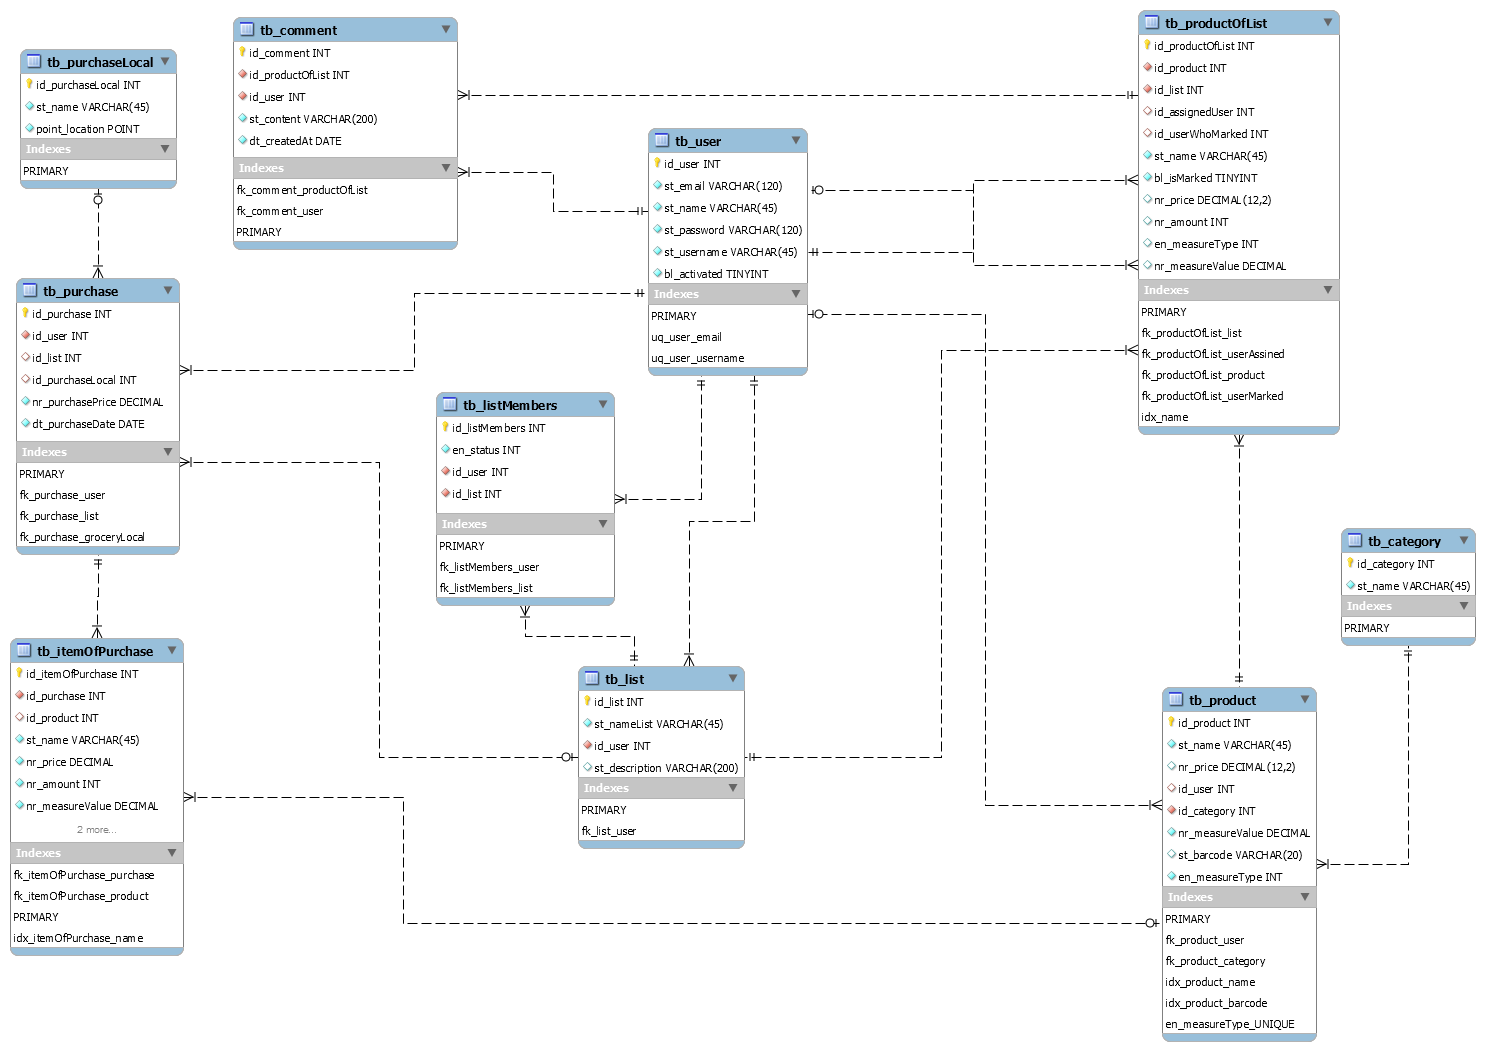
\includegraphics[scale=0.3]{mer}
  \legend{Fonte: Os autores}
\end{figure}

No diagrama, uma lista possui vários usuário, e um usuário pode estar em várias listas, surgindo assim a necessidade da tabela intermediária membrosLista. Essa tabela intermediária possui um status, que pode ser "Aceitado", "Rejeitado" e "Aguardando Confirmação".

Um cliente pode fazer vários comentários no produto da lista, 
e um comentário é de um cliente.

Uma lista pode ter várias compras (pois uma lista pode ser feita ao decorrer de várias compras), onde uma compra é de um mercado e possui vários items.

Tanto um produto da lista quanto um item da compra é 
composto um produto (sendo produto uma tabela mais genérica, pois assim será possível gerar dados estatísticos de produtos mais genéricos sem nenhuma especificidade como, por exemplo, marca do produto), sendo que o produto pode ter uma categoria.

\subsubsection{Definição de Índices}

No MySQL, temos dois tipos de índices:

\begin{enumerate}
	\item \underline{Índice Primário}: Criado pelo MySQL automaticamente ao criar chaves primárias (primary keys - PK) ou campo UNIQUE.
	\item \underline{Índice Secundário}: Criado e manipulado durante a modelagem para otimização de queries.
\end{enumerate}	

Nesse sentido, foram definidos índices secundários para as chaves estrangeiras (foreign key - FK) e para as colunas que no qual serão buscada no frontend por meio de campos de busca.

\subsection{Padrão Arquitetural}

A arquitetura escolhida para o desenvolvimento do Lixt foi cliente-servidor (com React-Native e Spring, respectivamente). Nesse tópico, iremos abordar detalhadamente o desenvolvimento de cada serviço.

\begin{figure}[H]
  \centering
  \caption{Detalhamento da Arquitetura}
  \label{fig:diagrama-componentes-arquitetura}
  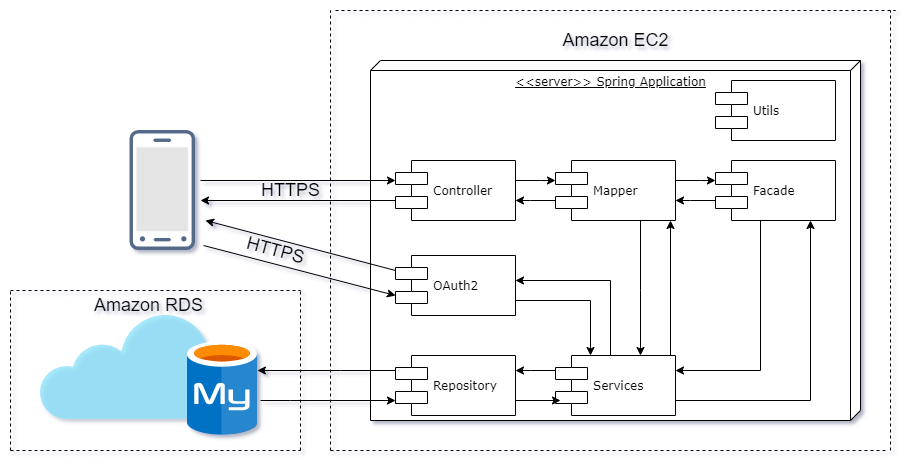
\includegraphics[scale=0.5]{diagrama-componentes-arquitetura}
  \legend{Fonte: Os autores}
\end{figure}

O cliente, que é uma aplicação mobile para Android, realizará requisições ao backend e, assim, conseguir operar suas funcionalidades e exibir os dados no layout de modo coerente no aplicativo.

O servidor, por sua vez, será dividida em camadas lógicas. A camada que será exposta e acessível para o frontend são os endpoints dos controllers, recebendo e retornando DTOs (padrão Data Transfer Object) em formato JSON. Após acessar o endpoint, caso esteja devidamente autenticado no OAuth2 e com o token de autorização, será chamado o mapper, responsável por converter DTO em model.

Após essa conversão, dependendo da complexidade da regra de negócio, pode chamar o service - para regras de negócios simple -  ou um facade - responsável por encapsular regras de negócios complexas, chamando os services a fim de evitar injeção de dependência cruzada entre os services. 

Os services, por sua vez, encapsulam as operações de CRUD do hibernate que são definidas nas Repositories.

Após a realização da requisição, será enviada uma resposta para o frontend, onde o mapper, dessa vez, irá converter o model em DTO, de modo que consiga tratar o dado a partir de formatações, retirada de dados sensíveis e garantindo maior performance ao enviar apenas os dados que serão devidamente utilizados (e não dados em excesso), garantindo menor dados em tráfego na rede, menor consumo de internet e maior velocidade.

O OAuth2 é o serviço de autenticação e autorização adotado que irá se aproveitar dos services para realizar a verificação das credenciais fornecidas no momento do login.

O Utils é uma biblioteca global que pode ser reutilizado em todo o projeto como, por exemplo, validação de dados, formatação de dados, entre outros.

O backend será hospedado no Amazon EC2 e o banco de dados MySQL estará disponível no Amazon RDS.
